%!TEX root = ../dissertation.tex

% : in primis, lo sviluppo di un backend in Ruby on Rails 5 completo delle funzionalità base per completare il flusso di operazioni da parte della farmacia e di API GraphQL per l'interazione con il \textit{front end}; in secondo luogo era prevista l'implementazione di API REST utilizzabile dal laboratorio di analisi, l'integrazione con le API del corriere SDA e la realizzazione di una suite di test completa; infine sarebbe avvenuta l'implementazione di requisiti facoltativi
\chapter{Introduzione}
\label{introduction}
\paragraph{}
Il presente documento espone il lavoro svolto dal laureando Andrea Trevisin durante il periodo di stage formativo presso Moku S.r.l. al fine di realizzare il \textit{back end} dell'applicazione web ``Biota'', una piattaforma per la gestione di esami della flora gastrointestinale.
Lo stage, della durata di 300 (trecento) ore, si è svolto tra il 15 maggio e il 17 luglio 2019 presso la sede di Roncade. Il progetto prevedeva il raggiungimento di diversi obiettivi, suddivisi in \textit{milestones}, a partire dalla realizzazione di un \textit{back end} completo delle funzionalità base della piattaforma, per poi implementare i requisiti opzionali e una suite di test completa e infine soddisfare alcuni requisiti desiderabili.
Al termine della durata dello stage, la piattaforma è in stato di produzione e tutti gli obiettivi sono stati soddisfatti.

\section{Azienda}
\paragraph{}
Moku S.r.l. è una startup nata nel 2013, con sede a Roncade (TV), fondata su un progetto software omonimo per una piattaforma web mirata a facilitare il lavoro condiviso su documenti di vario tipo. Si è poi evoluta diventando una società di consulenza IT che realizza prodotti software su commissione. 
Il team di Moku usa metodologie agili, basate su Scrum, e lavora a stretto contatto con il cliente; questo permette di individuare facilmente e velocemente i requisiti del prodotto, creando prodotti di qualità che rispecchiano le esigenze del committente. I principali ambiti di sviluppo di Moku sono piattaforme web applicazioni Android/IOS.

\begin{figure}[h!]
    
\includegraphics[width=\textwidth]{figures/logo_moku.png}
    \caption[Logo Moku]{Logo di Moku S.r.l.
    \label{fig:logomoku}}
\end{figure}    

\section{Processi aziendali}
\subsection{Modello di ciclo di vita del software}
\paragraph{}
Il modello di ciclo di vita del software adottato dal team di Moku si basa sulla metodologia Scrum. Scrum è un \textit{framework} agile per la gestione del ciclo di sviluppo del software, iterativo ed incrementale, creato e sviluppato da Ken Schwaber e Jeff Sutherland nel 1995; si propone di essere leggero, semplice da imparare ma difficile da padroneggiare. Scrum si presta bene alla modalità di lavoro di Moku, in quanto è ideato per team di dimensioni ridotte e permette di gestire progetti complessi offrendo la possibilità di reagire velocemente a cambiamenti. Una delle idee chiave è infatti la "volatilità dei requisiti", ovvero riconoscere che le esigenze dei clienti possano variare in corso d'opera, e che possano sorgere complicazioni non previste - specialmente quando si usano tecnologie all'avanguardia.

L'obiettivo principale è quindi la realizzazione di un prodotto software funzionante e soddisfacente a scapito di aspetti ritenuti non essenziali nell'immediato (e.g. una documentazione completa).

\subsubsection{Principi della metodologia Scrum}
\paragraph{}
Alla base del \textit{framework} vi è la teoria dei controlli empirici dell'analisi strumentale e funzionale di processo, altrimenti nota come "empirismo", la quale afferma che la conoscenza deriva dall'esperienza e le decisioni si devono basare su ciò che si conosce. L'implementazione dei controlli empirici di processo si basa su tre concetti:
\begin{itemize}
    \item \textbf{Trasparenza}: gli aspetti significativi del processo devono essere visibili ai responsabili del prodotto; la trasparenza richiede che tali aspetti siano definiti secondo uno standard comune in modo che gli osservatori condividano una comprensione comune di ciò che avviene.
    \item \textbf{Ispezione}: chi usa Scrum deve ispezionare spesso i prodotti della metodologia e il progresso verso l'obiettivo di uno \textit{sprint} per individuare eventuali difformità; tuttavia tale processo non dovrebbe essere frequente al punto da rallentare il lavoro. Le ispezioni danno il massimo beneficio quando eseguite da ispettori qualificati.
    \item \textbf{Adattamento}: se un'ispezione determina che uno o più aspetti sono al di fuori di certi limiti, e che il prodotto risultante è inaccettabile, il processo o il prodotto del processo vanno adattati; l'adattamento deve avvenire il prima possibile per evitare ulteriori difformità.
\end{itemize}

\subsubsection{Sprint}
\paragraph{}
Scrum prevede di dividere il progetto in blocchi contigui di lavoro, denominati \textit{sprint}, che prevedono un incremento del prodotto software rilasciabile al termine di ciascuno di essi.
Uno \textit{sprint} dura da 1 a 4 settimane, ed è preceduto da una riunione di pianificazione (\textit{sprint planning}) in cui vengono discussi e definiti obiettivi e stimate le tempistiche. Gli obiettivi stabiliti per uno \textit{sprint} possono variare solo allo \textit{sprint planning}successivo; ogni giorno viene fatta una breve riunione, detta \textit{daily scrum}, in cui viene brevemente discusso il lavoro da svolgere.

Nel corso di uno \textit{sprint}, il team realizza incrementi completi del prodotto: l'insieme di funzionalità inserite in un dato \textit{sprint} sono definite nel \textit{product backlog}, una lista ordinata di requisiti del prodotto che copre l'intero progetto. I requisiti scelti per essere soddisfatti durante un determinato sprint vanno a costituire \textit{sprint backlog}.

Gli \textit{sprint} in Moku durano generalmente 10/15 giorni, seguiti da una fase di valutazione del progresso rispetto alle aspettative e di pianificazione dello \textit{sprint} successivo, in cui viene stabilito il nuovo \textit{sprint backlog}. Dato il disaccoppiamento tra \textit{back end} e \textit{front end} nel progetto, i requisiti erano separati in due \textit{backlog differenti}.

\begin{figure}[h!]
    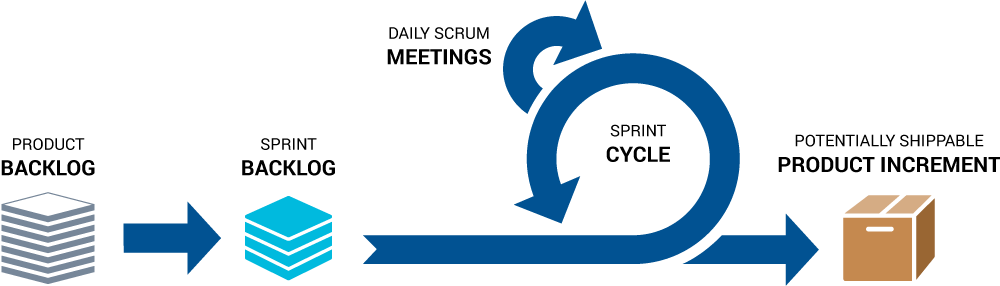
\includegraphics[width=\textwidth]{figures/agile-development-process.png}
    \caption[Scrum]{Rappresentazione grafica della metodologia Scrum
    \label{fig:scrum}}
\end{figure}    

\subsubsection{Ruoli di un team Scrum}
\indent Il \textit{framework} Scrum prevede che i team siano auto-organizzati, ovvero in grado di scegliere autonomamente il modo migliore per portare a termine il lavoro, e interfunzionali, cioè che non dipendono da altri o da parte del team per realizzare il prodotto. I team Scrum lavorano in maniera iterativa ed incrementale, massimizzando le possibilità di feedback utile. 

In un team Scrum sono presenti i seguenti ruoli:
\begin{itemize}
    \item \textbf{Product Owner}: responsabile della massimizzazione del valore del prodotto, rappresenta la "voce" degli stakeholders; definisce gli \textit{item} in base alle \textit{user stories} del cliente, ne assegna la priorità e li aggiunge al \textit{product backlog}.
    \item \textbf{Team di sviluppo}: responsabile della consegna del prodotto, con funzionalità incrementali e rilasciabile al termine di ogni \textit{sprint}; generalmente composto da 3-9 persone con competenze interfunzionali, che realizzano il prodotto effettivo.
    \item \textbf{Scrum Master}: responsabile della rimozione degli ostacoli che intralciano il team di sviluppo nel raggiungimento degli obiettivi dello \textit{sprint}; aiuta il team di sviluppo a comprendere e mettere in pratica la metodologia Scrum, assumendo un ruolo di "\textit{servant/leader}".
\end{itemize}

Per la durata dello stage, nonostante le linee guida di Scrum lo sconsiglino, i ruoli di \textit{Product Owner} e \textit{Scrum Master} erano ricoperti entrambi dal tutor aziendale per praticità. Il team di sviluppo, composto da due persone, includeva il laureando, il tutor aziendale (che interveniva solo ove fossero necessarie correzioni minori) e uno/due sviluppatori \textit{front end} (a seconda della disponibilità).

\subsection{Strumenti a supporto dei processi}
Per quanto riguarda gli strumenti di supporto ai processi, Moku usa per la maggior parte prodotti appartenenti all'ecosistema Atlassian, ottenendo una maggiore integrazione tra gli strumenti.

\subsubsection{Project management}
Per quanto riguarda la gestione dei progetti, Moku fa affidamento a Jira, un prodotto proprietario di Atlassian. Jira è uno strumento estremamente versatile che offre funzioni di \textit{issue tracking}, \textit{project management} e \textit{bug tracking}. Jira è inoltre fortemente orientato all'utilizzo della metodologia Scrum, permettendo di creare degli \textit{sprint} e di gestire il rispettivo \textit{backlog}.
\begin{itemize}
    \item \textbf{Issue tracking}: in Jira è possibile creare \textit{issue} di tipo \textit{Task} per compiti da completare, \textit{Story} per nuove (\textit{user stories}) e \textit{Feature/Improvement} per funzionalità o miglioramenti a funzionalità esistenti. Ogni \textit{issue} può essere assegnata ad uno o più membri del team, che può aggiornarne il progresso, dividerla in \textit{sub-task} e registrare le ore di lavoro. 
    \item \textbf{Enterprise resource planning}: Jira mette a disposizione uno strumento di pianificazione della distribuzione delle risorse temporali ed economiche, sotto il nome di \textit{Tempo}; esso permette di pianificare in anticipo il lavoro da dedicare ad una certa \textit{issue} per ogni membro del team, nonché di tenere traccia dei budget assegnati al progetto.
    \item \textbf{Bug tracking}: in Jira avviene creando issue di tipo \textit{Bug}.
\end{itemize}
Jira mette a disposizione un'interfaccia \textit{drag-and-drop}, che ne rende l'uso veloce ed intuitivo.

\begin{figure}[h!]
    \includegraphics[width=\textwidth]{figures/Jira.png}
    \caption[Jira]{Interfaccia della sezione di issue tracking di Jira
    \label{fig:Jira}}
\end{figure}    

\subsubsection{Gestione del versionamento}
Per la gestione del versionamento del prodotto software Moku usa \textit{repository Git} sul servizio di hosting Bitbucket, parte dell'ecosistema Atlassian. Bitbucket offre la possibilità di creare gratuitamente \textit{repository} private, risultando una scelta migliore per l'azienda. Queste vengono gestite localmente tramite il client dedicato Sourcetree, anch'esso proprietario di Atlassian (quindi perfettamente integrato con Bitbucket), il quale semplifica l'uso del paradigma \textit{git-flow}, scelto come standard da Moku.

\subsubsection{Gestione delle comunicazioni}
\paragraph{A livello aziendale} La corrispondenza riguardante l'avvio del progetto di stage e la collaborazione con il cliente, così come altre comunicazioni a livello aziendale, sono avvenute tramite posta elettronica.
\paragraph{Nel team} Per facilitare la comunicazione tra i membri di ogni team di sviluppo, nonché per comunicazioni meno importanti, Moku fa uso di Slack. Slack è un applicativo \textit{cloud-based} di messaggistica e file-sharing, in cui i messaggi vengono inviati in "canali": questo permette di dividere le comunicazioni per progetto, facilitando anche la ricerca di informazioni rilevanti precedentemente inviate.

\section{Organizzazione del testo}

\section{Convenzioni tipografiche}
